\documentclass[12pt,conference,compsoc]{IEEEtran}

\ifCLASSOPTIONcompsoc
  \usepackage[nocompress]{cite}
\else
  \usepackage{cite}
\fi

\ifCLASSINFOpdf
\usepackage[pdftex]{graphicx}
\else
\usepackage[dvips]{graphicx}
\fi
\usepackage{url}
\hyphenation{op-tical net-works semi-conduc-tor}

\begin{document}
\title{A Study of Cuckoo Hashing}
\author{\IEEEauthorblockN{Zhijia Chen}}
\maketitle
\IEEEpeerreviewmaketitle

\section{Introduction}
It is said that the data are to this century what oil was to the last one: a driving force of growth and change. Indeed, data has been acting as fuels for many techniques such as machine learning , the Internet of Things and big data analysis, which in turn promote people to generate even more data. The data in last few decades has been growing exponentially and is supposed to keep the exploding trend. According to the report of International Data Corporation (IDC) published in 2014, the total size of data in the digital universe will reach to 44 zettabytes by 2020, and nearly 50\% of cloud-based services will rely on data in storage systems~\cite{IDC}. What's more, many computing devices, from small IoT sensors to powerful server in large scale data centers, are collecting and analyzing ever-greater amounts of data. A users in routine generate queries on hundreds of Gigabytes of data stored in their local storage or cloud storage systems, and commercial companies generally handle Terabytes and even Petabytes of data each day~\cite{IDC}.

With the exponential growing trend of data, it is more and more challenging for cloud storage systems to serve queries in a real-time manner and keep a stable throughput over time, which consumes substantial resources to support query-related operations~\cite{SmartCuckoo}. And effective hashing scheme is becoming a critical factor for query service to keep up with the data growth. A hash table maps a keys to values and it uses a hash function to compute the position in the table where the corresponding data could be stored or found. Hash tables are so adorable for data indexing because they have a constant lookup complexity on average which supports fast query response whatever the data size is. But hash table has also has its drawback --- hashing collision. Because a hash function usually maps multiple distinctive elements into one element, it may points multiple different keys to the same slot. So one of the most basic tasks when designing a hashing scheme is to handle hashing collision. Generally there are three strategies for resolving hashing collisions~\cite{cuckooTutorial}:

\begin{itemize}
    \item \textbf{Perfect hashing:} Choose a hash function with no collisions. The idea of using hashing functions that prevent the collisions seems appealing. However, it requires complete knowledge of all the keys to construct a perfect hashing function~\cite{perfectHashing}, which is not feasible for large cloud data storage centers that need to handle new coming data all the time.

    \item \textbf{Open addressing:} Allow items to overflow out of their target bucket and into other paces. With open addressing, data collisions are resolved by finding alternative locations in hash table by probing a sequence of possible indices. Suppose $T_i$ is the $i$th probing position and $h(x), h_1(x), h_2(x)$ are hash functions, three basic probing methods are listed below.
    \begin{itemize}
        \item Linear probing: $T_i(x)=h(x)+i$
        \item Quadratic probing: $T_i(x)=h(x)+i^2$
        \item Double hashing: $T_i(x)=h_1(x)+i\times h_2(x)$
    \end{itemize}

    \item \textbf{Closed addressing (separate chaining):} All the colliding items should be stored in the target bucket with the help of some auxiliary data structures. The closed addressing (also called separate chaining) resolves hashing collision by storing all colliding items in an auxiliary linked list or BST. The basic implementation are simple, but its performance is sensitive to data distribution, as a lookup in a bucket with collisions will involve a searching the auxiliary data structure, which could be very expensive in some unfortunate cases where too much keys are collided in the bucket due to skewed distribution of data.
\end{itemize}


Both open addressing and closed addressing, however, will suffer from great latencies when there are too many collisions in the target bucket under some unfortunate cases. So people are looking for hashing schemes that could have a constant lookup time even in the worst case, and cuckoo hashing is one of those candidates. Cuckoo hashing is a fast and simple hashing scheme with constant-time worst-case lookup ($O(ln\frac{1}{\epsilon})$) and has $(1+\epsilon)n$ memory consumption, where $\epsilon$ is a small constant~\cite{cuckoo}. It is widely used in large storage systems for its desirable properties. Unlike simple hashing schemes that provide only one bucket, cuckoo hashing provides $N$ ($N=2$ in common practice) possible locations for each item by using $N$ hash functions to reduce the change of collision. And to resolve collisions, old items are kicked out by the new comers and turn to their alternate buckets. To look up for an item, the cuckoo hashing only needs to search for a small number of buckets (depends on the number of hash functions being used), which is a constant time even under the worst case.

However, cuckoo hashing suffers from substantial performance penalty during insertion when the recursively kicking out operation turn out be an endless loop. The endless loop indicates a failure for insertion and need to perform a rehashing in order to accommodate all items. The endless loop itself, while useless for the result, consumes lots of time and resources, and it's only after exhaustive attempts the cuckoo hashing could realize that it's endless and perform rehashing, which leads to non-deterministic performance and is not desirable for cloud storage systems that are supposed to handle queries in real-time manner. 

This paper presents the basic cuckoo hashing and some of its state-of-the-art variants that addressed on its non-deterministic performance issue during insertion. The rest of the paper is organized as follows. In section~\ref{sec:cuckoo}, we present the basic cuckoo hashing and illustrate its operations with some examples. We describe three cuckoo hashing variants---cuckoo hashing with a stash (CHS), SmartCuckoo and horton tables---in the following three sections, and then we compare the three variants and conclude in section 6.

\section{Standard Cuckoo Hashing}
\label{sec:cuckoo}
The standard cuckoo hashing scheme was proposed by Pagh and Rodler in [cuckoo hashing]. Suppose we attempt to accommodate $n$ items with two tables, $T_1$ and $T_2$, each has $\frac{n}{2}$ buckets and one hash function ($h_1$ for $T_1$ and $h_2$ for $T_2$). Each bucket can store at most one item. To insert an item $x$, we place it in $T_1[h_1(x)]$ if that bucket is empty. Otherwise (suppose it is taken by item $a$), we kick out $a$ in $T_1[h_1(x)]$ and replace it with $x$, then we try to insert $a$ into $T_2[h_2(a)]$. If $T_2[h_2(a)]$ is empty, then we are done, and if it is not (suppose it is taken by item $b$), then we further replace $b$ with $a$ and turn $b$ to bucket $T_1[h_1(b)]$ and so on, bouncing between $T_1$ and $T_2$ until all items stablize.

Inserting item $x$ will end up in one of the following three cases, as illustrated in Fig.~\ref{fig:cuckoo-example}. The directed edges beween the two tables gives the potential postions of the items. Each edges points from one item's actually storage location to its alternative location.

\begin{itemize}
    \item Item $x$ is inserted without any kick-out operation. As shown in Fig.~\ref{fig:cuckoo-example}(a), two items ($a$ and $b$) are initially stored in $T_1$ and $T_2$. When inserting $x$, its twp candidate buckets are $T_1[0]$ and $T_2[5]$. $T_1[0]$ is occupied by item $a$ while $T_2[5]$ is empty, so we place $x$ in $T_2[5]$ and add an edge directed from $T_2[5]$ to $T_1[0]$.
    \item Item $x$ is inserted with finite kick-out operations. As shown in Fig.~\ref{fig:cuckoo-example}(b), items $c$ and $d$ are inserted into the hash tables before $x$. The two candidate bucket of $x$ are occupied by $a$ and $d$ respectively. To accommodate $x$, we kick out $a$ and move it to $T_2[1]$, which further moves $b$ to $T_1[2]$. This procedure is repeated until en empty bucket is found at $T_2[3]$. The kick-out path is $x\rightarrow a\rightarrow b\rightarrow c$.
    \item Inserting item $x$ runs into infinite kick-out operations. As shown in Fig.~\ref{fig:cuckoo-example}(b), items $e$ is inserted into the hash tables before $x$. There is no vacant bucket to accommodate $x$ even after substantial kick-out operations, which results in an endless loop. The cuckoo hashing has to carry out a rehashing operation~\cite{cuckoo}.
\end{itemize}

\begin{figure}
    \centering
    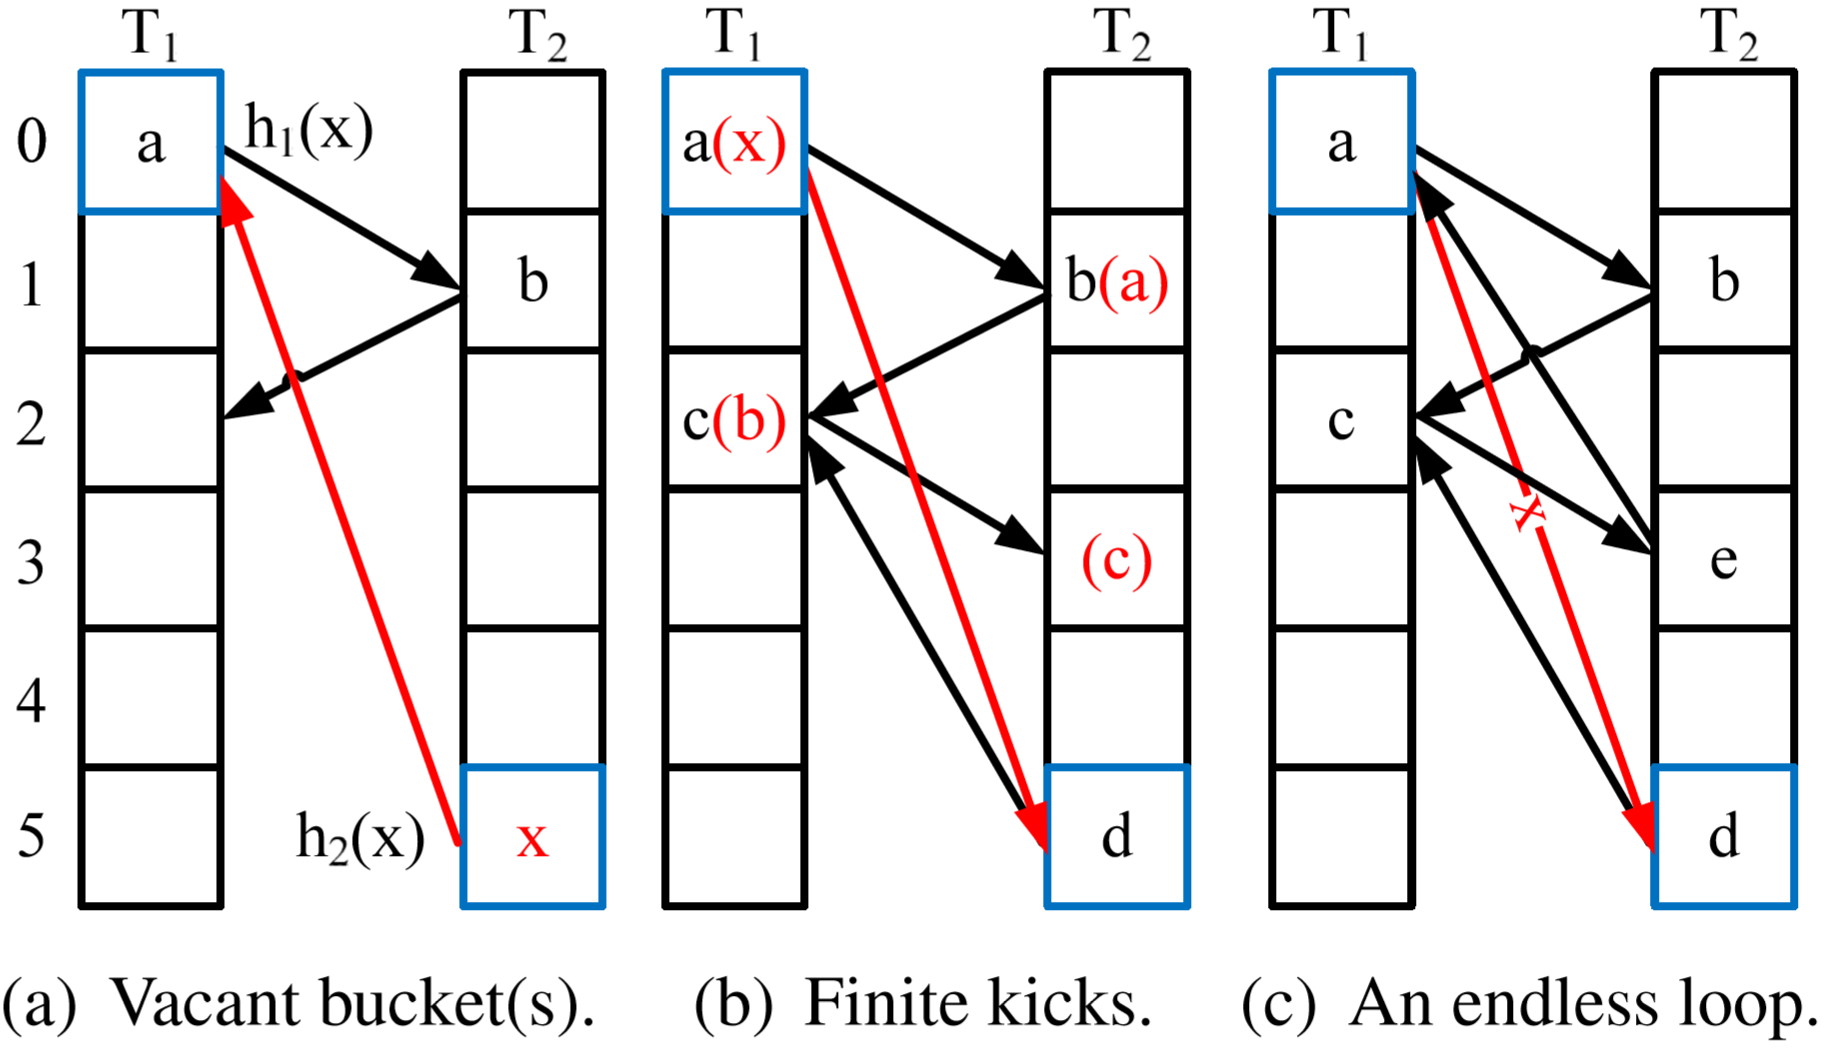
\includegraphics[width=\linewidth]{fig1.png}
    \caption{The standard cuckoo hashing data structure.
    } \label{fig:cuckoo-example}
\end{figure}

A lookup or delete operation only needs to probes the two candidate buckets of an item, which requires a constant time. For example, to query $x$, we only need to check $T_1[0]$ and $T_2[5]$ as shown in Fig.~\ref{fig:cuckoo-example}.

If the two hash functions are chosen independently from an appropriate universal hash family, then we can expect to insert all $n$ items successfully with at most $\alpha logn$ kick-out operations for any particluar item with probability $1-O(1/n)$, and $\alpha$ is a sufficiently large constant. Further more, if we limit the number of kick-out operation to $\alpha logn$ before rehashing, then the expected time to insert all $n$ items successfully into the table is $O(n)$, which means the expected insert complexity of the standard cuckoo hashing is also a constant~\cite{cuckoo}.

\section{Cuckoo Hashing with a Stash}
\label{sec:chs}
Cuckoo hashing supports simple worst-case $O(1)$ lookups, however, collisions are still troublesome for insertion. Though rare, there is always a chance that on the insertion of a new item, we could not find a place to hold the item even after substantial attempts, causing a failure. In such case, a full rehash is required to find new hash functions to accommodate all items appropriately. Theoretically speaking, the insertion failure of cuckoo hashing happens with a low probability ($O(n^-c)$ for some constant $c\geq 1$). The rehashing has very limited impact on the average query performance, but the very existence of those unfortunate chances make it hard to guarantee the performance. Moreover, the constant $c$ in $O(n^-c)$ failure probability bound is hard to be measured thus difficult to guarantee that $c$ is above the desirable level in practice. For example, values of $c\leq3$ may lead too much failure of commercial applications.

Cuckoo hashing with a stash (CHS) is a variant of cuckoo hashing that utilizes a small amount of memory to construct a small stash out side the main hash tables. Specifically, by storing a constant number of items outside the table in an area that called stash, we can dramatically reduce the probability of insertion failure where a rehash operation is necessary. The intuition behind the approach is that, if items cause insertion failure independently, then we can expect the number of items that cause insertion failure to be \textbf{$P_r$}$(S\geq s)=O(n^{-cs})$ for some constant $c>0$ and every constant $s\geq 1$. And we can identify those problematic items during insertion and store them in the stash, dramatically reducing the failure probability bound[CHS].

\begin{figure}
    \centering
    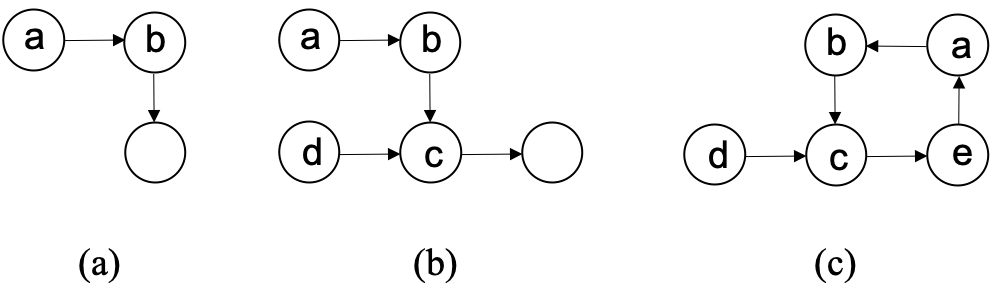
\includegraphics[width=\linewidth]{cuckoo-graph.png}
    \caption{The corresponding cuckoo graph of Fig.~\ref{fig:cuckoo-example}
    } \label{fig:cuckoo-graph}
\end{figure}

To detect the problematic item, CHS relies on \textit{cuckoo graph} which is a multi-graph that derived from the two hash tables of cuckoo hashing. The graph corresponding to the Fig.~\ref{fig:cuckoo-example} is shown in Fig.~\ref{fig:cuckoo-graph}. In a cuckoo graph, each vertex represents an alternative bucket of some items (no matter the bucket is actually occupied or not), and each directed edge corresponds to an item and is directed from its actual stored bucket to its alternative bucket. Note that the cuckoo graph can only represent cuckoo hashing that has two hash functions. We can easily determine if an insertion would fail or not with the help of cuckoo graph. Since each vertex has at most one outgoing edge, each component in a cuckoo graph has at most one cycle. Inserting a new element will add a new edge in the graph, and if the target vertex is connected to a cycle, then the insertion is doomed to fail[Cuckoo Hashing: Further Analysis. Information Processing Letters]. During insertion, the CHS will put an item in the stash whose corresponding edge belongs to a cycle, thus avoids insertion failure. And the items in the stash will be inserted into the hash tables late whenever there are available buckets. So a rehash is only needed when the stash is full and none of the items in the stash could be successfully inserted into the tables without rehashing.

There are many ways to implement the insertion algorithm for CHS. One way is to track the bucket that has been visited during insertion. During a successful insertion, at most one vertex of the cuckoo graph is visited (kicking out the item in the corresponding bucket) more than once, and no vertex is visited more than twice. Thus we can remember the slots that has been visited during the insertion, and when a bucket has been visited more than twice, put the item into the stash. However, logging the buckets that has been visited could be expensive, thus the author suggests that we set a limit of $\alpha logn$ on the number of possible kick-out operations. And if $\alpha logn$ evictions do not suffice to settle down, then we 'roll back' to the original configuration and try to insert the new coming item second time with the 'cycle detection' mechanism~\cite{CHS}.

\cite{CHS} has proved that for every constant integer $s\geq 1$, for a sufficiently large constant $\alpha$, the size $S$ of the stash after all items have been inserted satisfies \textbf{$P_r$}$(S\geq s)=O(n^{-s})$.


\section{SmartCuckoo}
\label{sec:smart}
Many cuckoo hashing variants have addressed the problem of endless kickout operations when countering an insertion failure. The common feature of them is to set an upbound on the number of evict operations before performing rehashing. However, those kick-out loops executed in failure insertion consume substantial rescources and they are just fruitless efforts. The insertion performance of cuckoo hashing will be much better if we can identify the endless loops and avoid wasting time and resources on them. With such motivation, \textit{SmartCuckoo} is designed to predetermine and identify endless loops during insertion. Like CHS, \textit{SmartCuckoo} also leverages on the cuckoo graph to identify the cycles. However, instead of remembering visited buckets to track the component of cuckoo graph that involved in current execution, \textit{SmnartCuckoo} builds an extra directed pseudoforest graph structure to present the entire cuckoo graph. Then for each insertion, \textit{SmartCuckoo} checks if the new item will add an edge to an existing cycle, and thus predetermine if the insertion can succeed or not.

In SmartCuckoo, a directed graph in which each vertex has an outdegree of exactly one is defined as a \textbf{maximal directed pseudoforest}, and a subgraph of the pseudoforest that has the same number of vertices and edges are named \textbf{maximal subgraph}. A maximal subgraph contains a cycle, as the outdegree of each vertex is at most one. Fig.~\ref{fig:maximal-graph}(a) shows an example of a maximal directed pseudoforest, and there are three maximal subgraphs in the pseudoforest, while Fig.~\ref{fig:maximal-graph}(b) shows an example of non-maximal directed pseudoforest which contains two non-maximal subgraphs. 

\begin{figure}
    \centering
    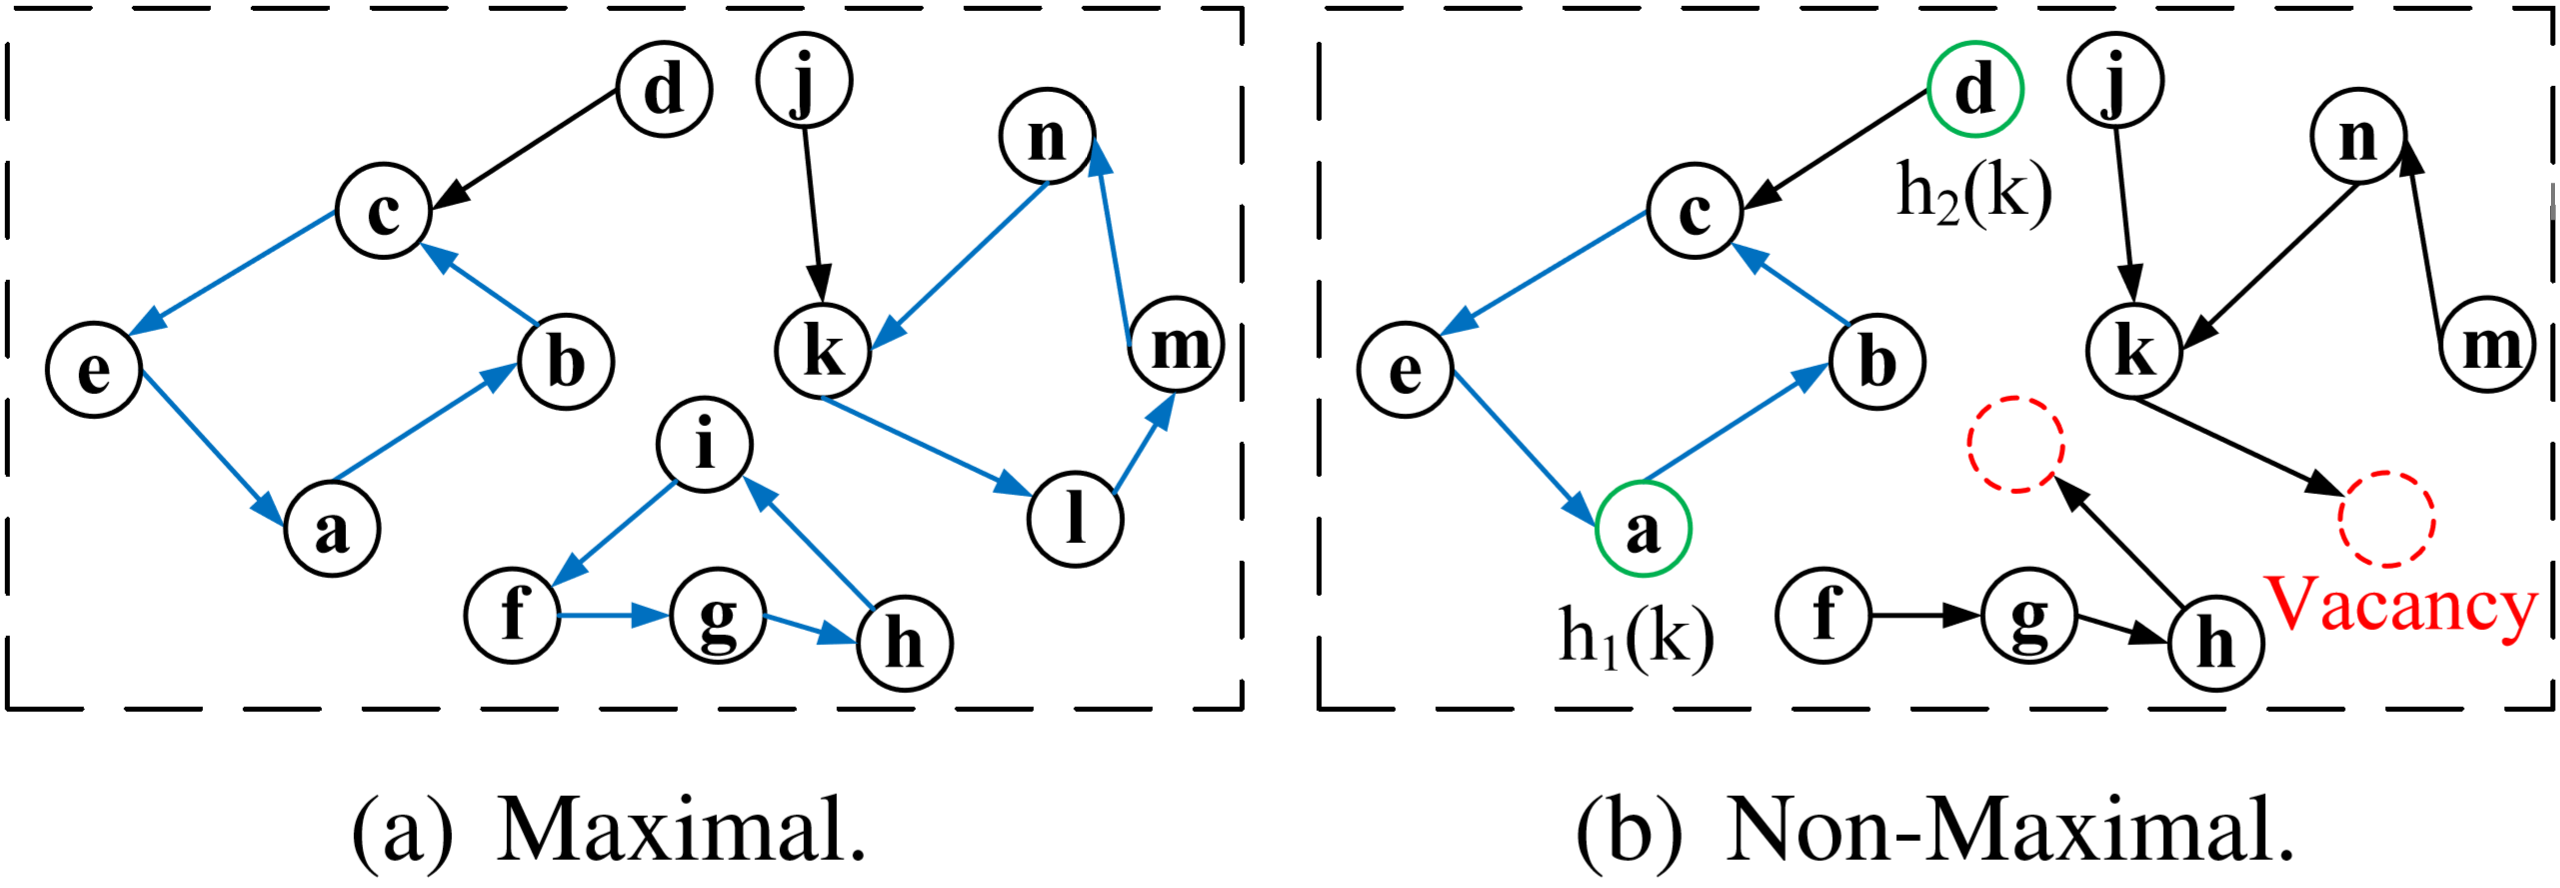
\includegraphics[width=\linewidth]{maximal-graph.png}
    \caption{The directed pseudoforest.} \label{fig:maximal-graph}
\end{figure}

In a directed pseudoforest, each vertex corresponds to a bucket, and each edge corresponds to an item and is directed from the its actual store bucket to its alternative bucket. Thus each insertion will add a new edge to the pseudoforest, and add zero, one or two vertices, depending on the two buckets are taken or not.  \textit{SmartCuckoo} classifies items insertions into the following three cases based on the number of additional vertices added to the directed pseudoforest, and with help of the directed pseudoforest which tracks the item placements, it can accurately predict the occurrence of endless loops.

\begin{figure}
    \centering
    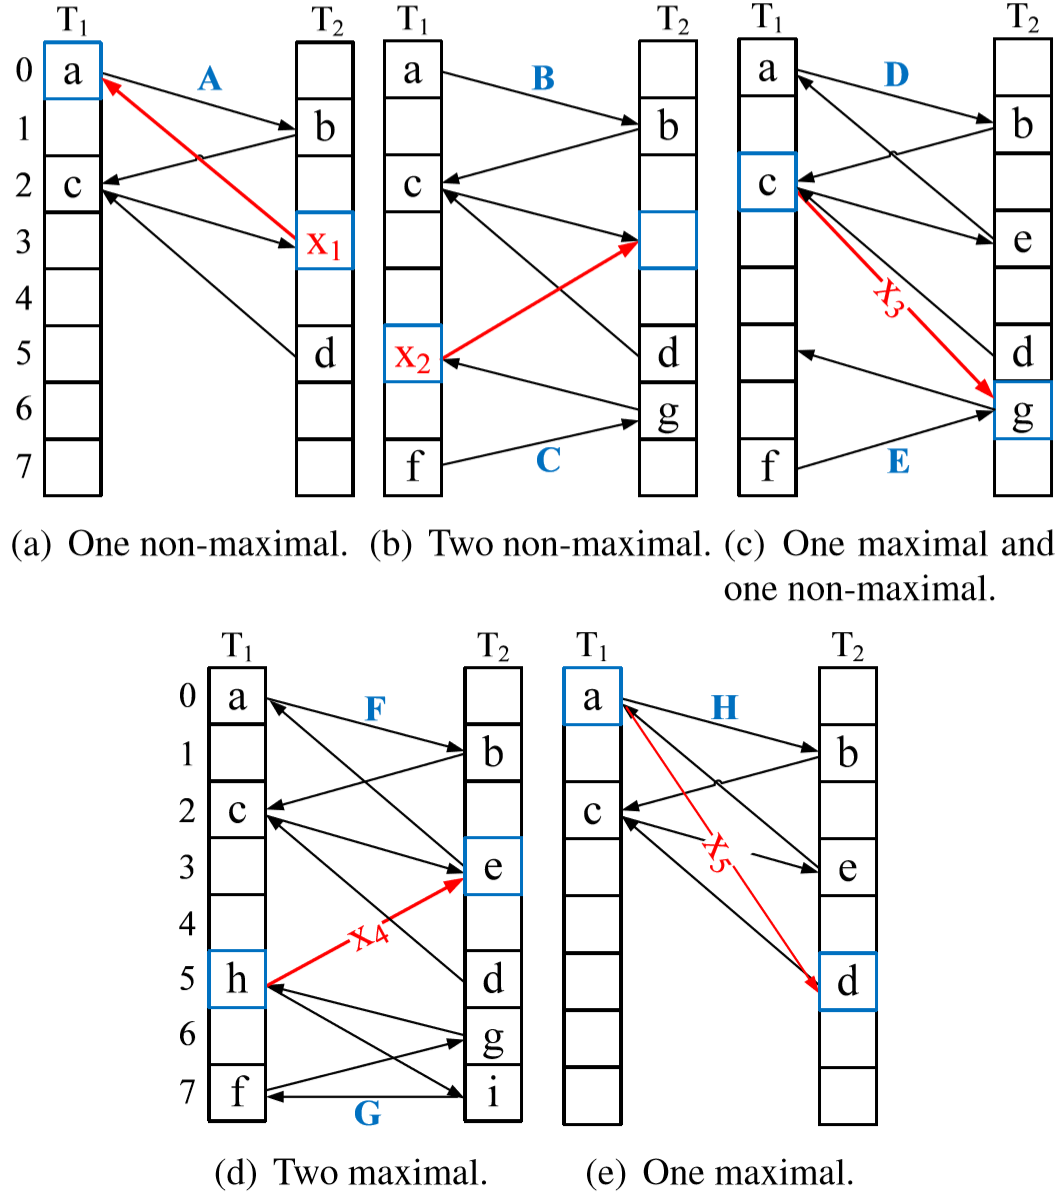
\includegraphics[width=\linewidth]{v+0.png}
    \caption{Five scenarios for Case $v+0$.} \label{fig:v+0}
\end{figure}

\begin{figure}
    \centering
    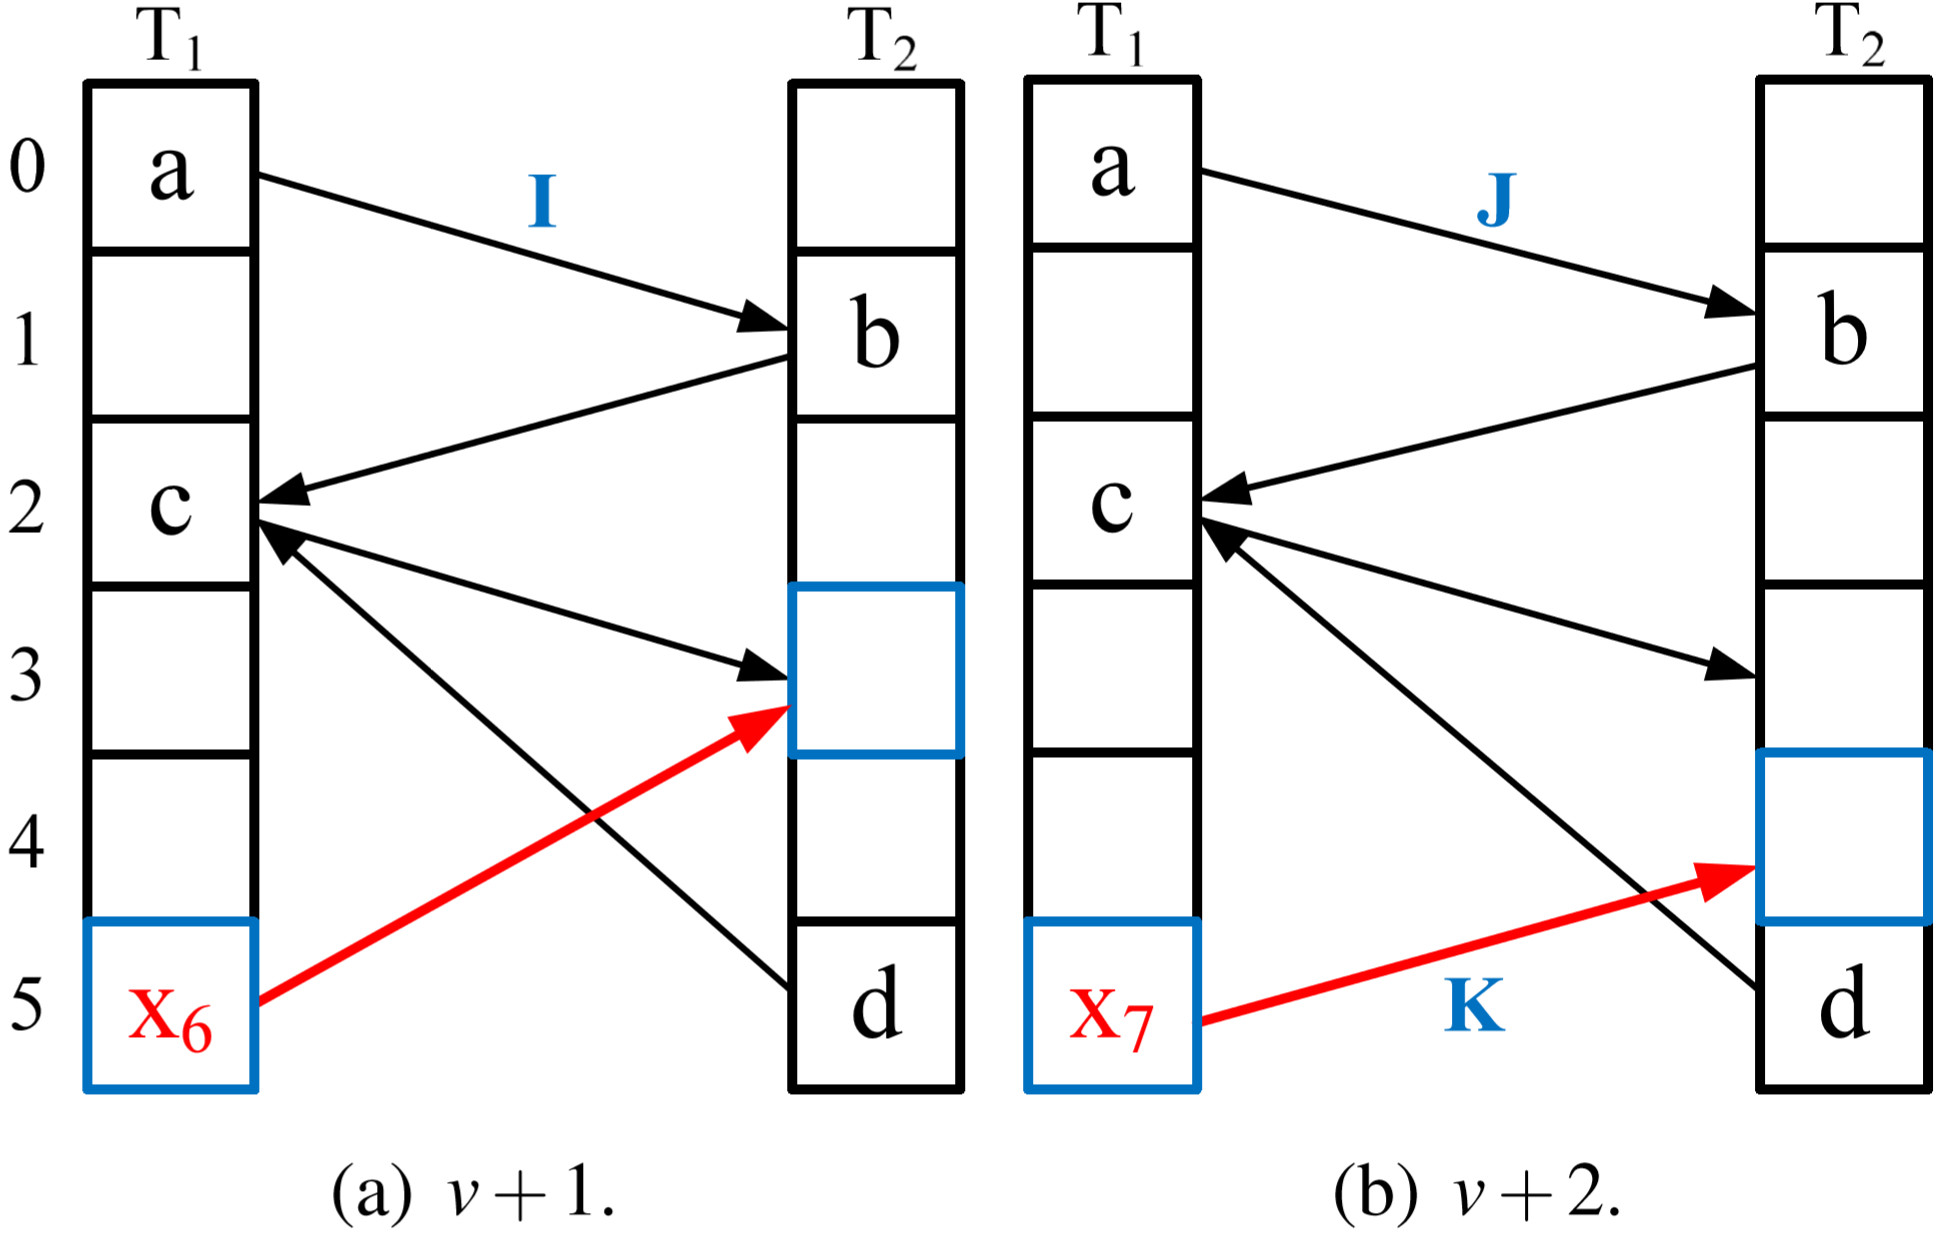
\includegraphics[width=0.7
    \linewidth]{v+1-2.png}
    \caption{Five scenarios for Case $v+1$ and $v+2$.} \label{fig:v+1-2}
\end{figure}

\begin{itemize}
    \item \textbf{The Case of $v+0$}: When inserting item $x$, if the two buckets given by $h_1(x)$ and $h_2(x)$ are both occupied, then the insertion will not add new vertex to the pseudoforest. And this case have five possible scenarios, as illustrated by Fig.~\ref{fig:v+0}.
    \begin{itemize}
        \item The two candidate buckets of item $x_1$, showns as blue buckets in Fig.~\ref{fig:v+0}(a), already exist in the same non-maximal subgraph $A$. Either bucket can be used to place $x_1$, as the kick-out operation will finally find an empty bucket in the subgraph.
        \item The two candidate buckets of item $x_2$ already exist in two non-maximal subgraph $B$ and $C$ respectively, as shown in Fig.~\ref{fig:v+0}(b). The insertion will success as both $B$ and $C$ have vacant bucket.
        \item One candidate bucket of item $x_3$ is in the non-maximal subgraph $E$ and the other is in the maximal subgraph $D$, as shown in Fig.~\ref{fig:v+0}(c). $x_3$ should be placed in the bucket in the non-maximal subgraph to avoid endless loops.
        \item The two candidate buckets of item $x_4$ already exist in two maximal subgraphs $F$ and $G$ as shown in Fig.~\ref{fig:v+0}(d). Inserting into either bucket will lead to endless loops.
        \item The two candidate buckets of item $x_4$ already exist in one maximal subgraph $H$ as shown in Fig.~\ref{fig:v+0}(e). Inserting into either bucket will lead to endless loops.
    \end{itemize}
    \item \textbf{The Case of $v+1$}: If one of the candidate bucket of item $x$ is occupied, i.e., it is in one subgraph, while the other is neither occupied nor a candidate bucket of any other items, inserting $x$ will add a new vertex to the subgraph, as illustrated by Fig.~\ref{fig:v+1-2}(a).
    \item \textbf{The Case of $v+2$}: If both the two candidate buckets of item $x$ have not been claimed by any other items, inserting $x$ will introduce a new subgraph that formed by the two candidate buckets to the pseudoforest, as illustrated by Fig.~\ref{fig:v+1-2}(b).
\end{itemize}

~\cite{SmartCuckoo} evaluated \textit{SmartCuckoo} and compared it with many other state-of-the-art cuckoo hashing variants---CHS, libcuckoo and bucketized cuckoo hash tables---in terms of insertion throughput, lookup throughput, and the throughput of mixed queries. The results showed that \textit{SmartCuckoo}'s insertion performance is significantly better than other variants. Specifically, compared to CHS, the insertion of \textit{SmartCuckoo} is 0.5 times to 5 times faster, increasing with table load factor, as shown in Fig.~\ref{fig:performance}. The reason is that, when table is heavier loaded, more insertion will be involved in endless loops, and the advantage of skipping those loops becomes more significant.

\begin{figure}
    \centering
    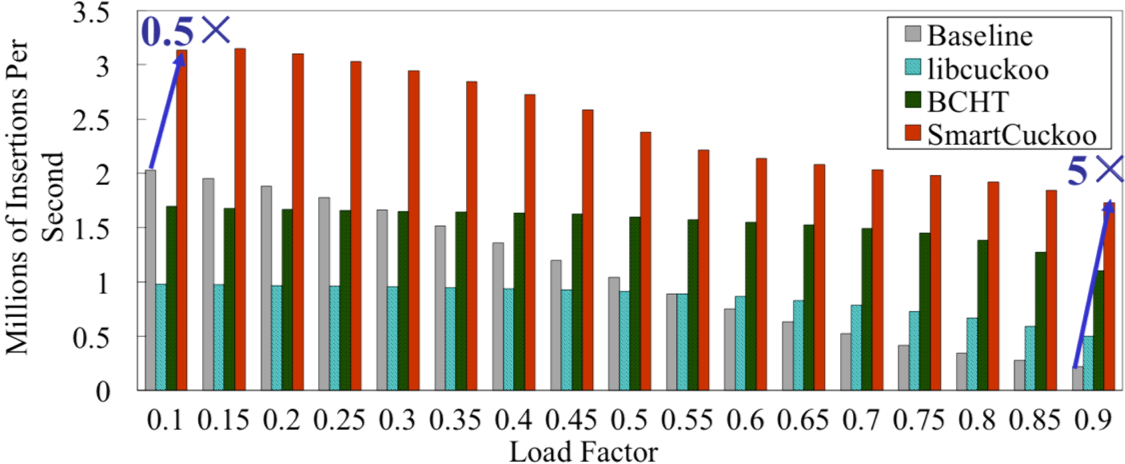
\includegraphics[width=\linewidth]{performance.png}
    \caption{Five scenarios for Case $v+1$ and $v+2$.} \label{fig:performance}
\end{figure}

\section{Bucketized Cuckoo Hash Table}
\label{sec:BCHT}
Bucketized cuckoo hash table (BCHT) is another variant of cuckoo hashing that, instead of storing only one items, it groups multiple cells into one buckets with each bucket typically has two to eight slots, and each slot capable of storing a single item. Like the the standard cuckoo hashing, BCHT also utilizes two hash functions, and during insertion, the new comming item is offered two buckets and it can be placed in either empty slot within the two buckets. In the case that neither bucket has empty slot to hold the item, BCHT repeats the same kick-out operations as standard cuckoo hashing, until an available slot is found, or after sufficient loops, performs rehashing. Compared to the standard cuckoo hashing, BCHT use a small lookup and deletion overhead to trade for a  higher throughput lookups and load factors that offer excedes 95\% with greater than 99\% probability~\cite{coolCuckoo}.

\begin{figure}
    \centering
    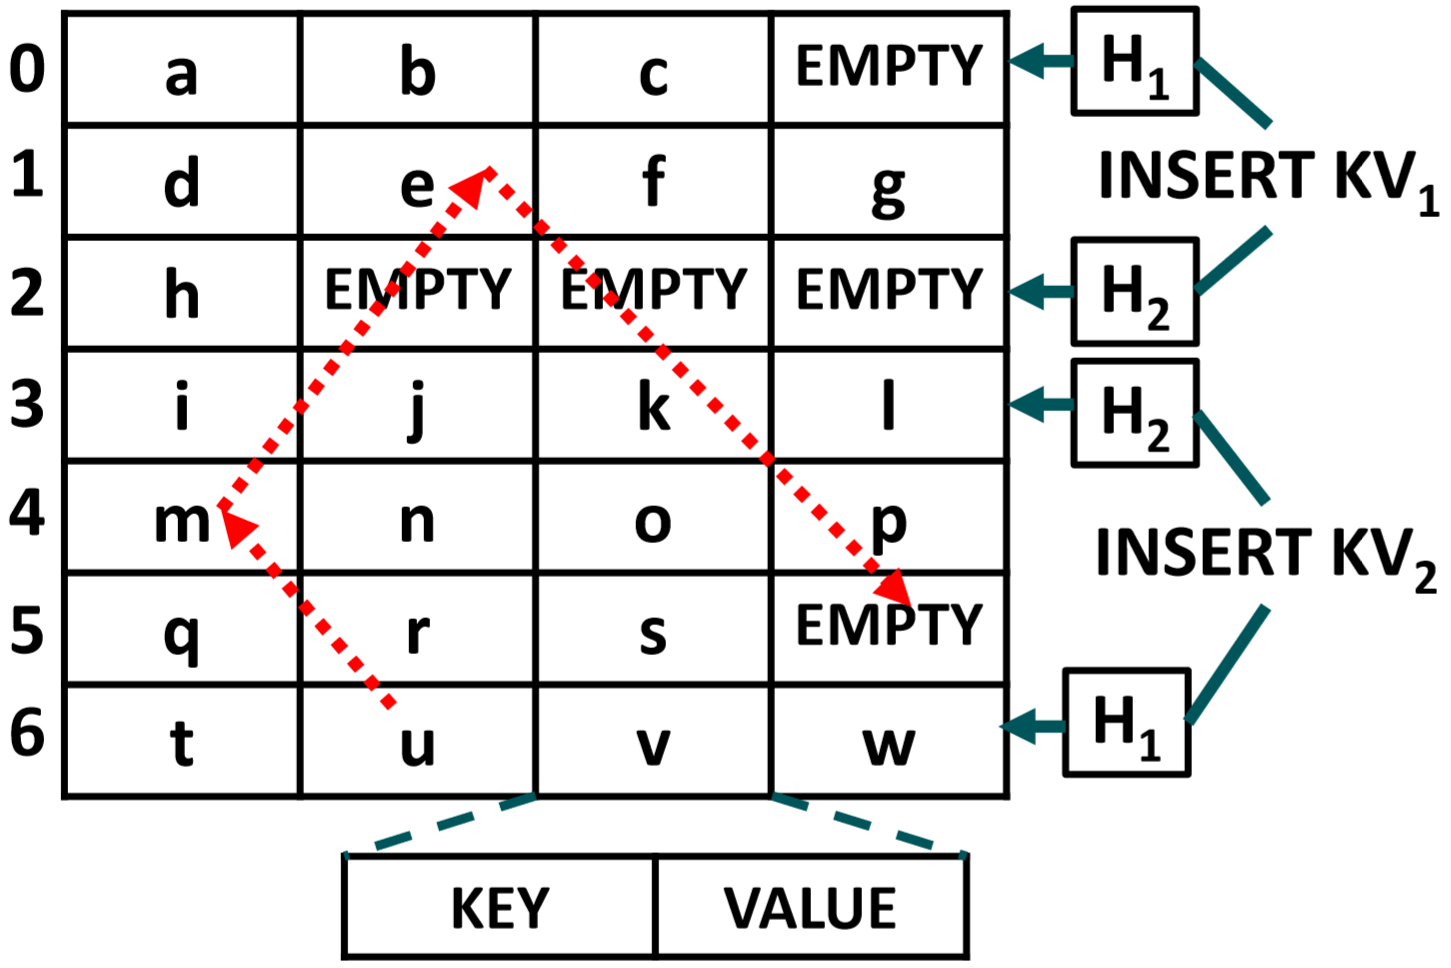
\includegraphics[width=\linewidth]{BCHT.png}
    \caption{Inserting items \textbf{KV1} and \textbf{KV2} into a BCHT.} \label{fig:BCHT}
\end{figure}

Figure.~\ref{fig:BCHT} illustrates the basic insertion operations of BCHT with two different key-value pairs $KV_1$ and $KV_2$. Each row in the figure is a bucket, and each bucket has 4 cells. The $H_1$ and $H_2$ are two independent hash functions that are used to hash each item to its two candidate buckets. For $KV_1$, the two candidate buckets are bucket 0 and bucket 2, while for $KV_2$ they are bucket 3 and bucket 6. $KV_1$ can be placed in either one of the candidates because both of them have empty slots, and it is up to the algorithm to decide with bucket to use. For $KV_2$, its two candidate buckets are both full, and kick-out operations are required to accommodate the item. In this case, item $u$ in the bucket 6 is evicted and replaces item $m$ in bucket 4, which then kick out item $e$ in bucket 1 and relocates $e$ to bucket 5. 

There are generally two methdos to lookup for an item in BCHT. The first method optimize latency, which always accesses all the candidate bucket of the expected item in parallel~\cite{li2014algorithmic}. The other technique, which optimizes bandwidth, avoids fetching additional buckets where feasible~\cite{memC3}.

Given $f$ independent functions where each of them maps an item to one candidate bucket, the latency-optimized method always checks all the $f$ buckets at the same time, while the bandwidth-optimized method always checks $f$ candidate buckets one by one and thus, touches $(f+1)2$ buckets on positive lookups and $f$ buckets on negative lookups.

When the bandwidth-optimized method is used in BCHT, the insertion policy would an impact on the lookup performance, because a bandwidth-optimized algorithm always searches the expected item's candidate buckets in certain order. If the expected item is found before searching the last of $f$ candidate buckets, then cost to search the remaining candidate buckets can be saved. If $f$ is 2, and $H_1$ and $H_2$ the first and second hash function used in the lookups, then the expected lookup cost across all inserted items is $1\times p+2\times (1-p)$, where p is the fraction of items that inserted using $H_1$. Therefore, the insertion algorithm's policy on when to use $H_1$ or $H_2$ affects the lookup cost. Generally, there are two insertion policies:

\begin{itemize}
    \item \textbf{Load-balancing policy:} Check the available slots of all the candidate buckets and place the new item into the bucket that has most empty slots. For example, if we use such policy in the example shown in Fig.~\ref{fig:BCHT}, then $KV_1$ should be placed in the bucket hashed by $H_2$. The intuition behind this load balancing policy is that it increase the possiblity of reaching a higher load factor before a rehashing is required, and since $H_1$ and $H_2$ are used with equal probability, 1.5 buckets are searched on average for positive lookups.
    \item \textbf{First-fit policy:} Always placed in the first available slot. For example, with the first-fit polcy, $KV_1$ in the example of Fig.~\ref{fig:BCHT} will be placed in the last slot in bucket 0, even though bucket 2 has more empty slots. This policy inserts items with fewer memory accesses by avoiding fetching unnecessary candidate buckets.
\end{itemize}

In the existing bandwidth-optimized BCHT implementations, the load-balancing policy is used to optimize the lookup costs, while the first-fit plicy is adopted for a better insertion performance.

\section{Horton Tables}
\label{sec:horton}
Horton tables is a cuckoo hashing variant derived from BCHT, which trades a small amount of space for achieving positive and negative lookups that expected to check close to 1 bucket[horton]. Horton tables construct two type of buckets (as illustrated in Fig.~\ref{fig:bucket-type}). The first type is the standard BCHT bucket (\textbf{type A})and the second (\textbf{type B}) contains auxiliary metadata that tracks the items that are primarily hashed to the bucket but have to be remapped to other buckets due to insuffcient capability of cells. In the initial state, all the buckets are type A buckets, and they will be transformed to type B buckets once they are overflow. Such design enabels Horton tables to track remapped items at a very low costs, both in terms of time and space~\cite{Horton}.

\begin{figure}
    \centering
    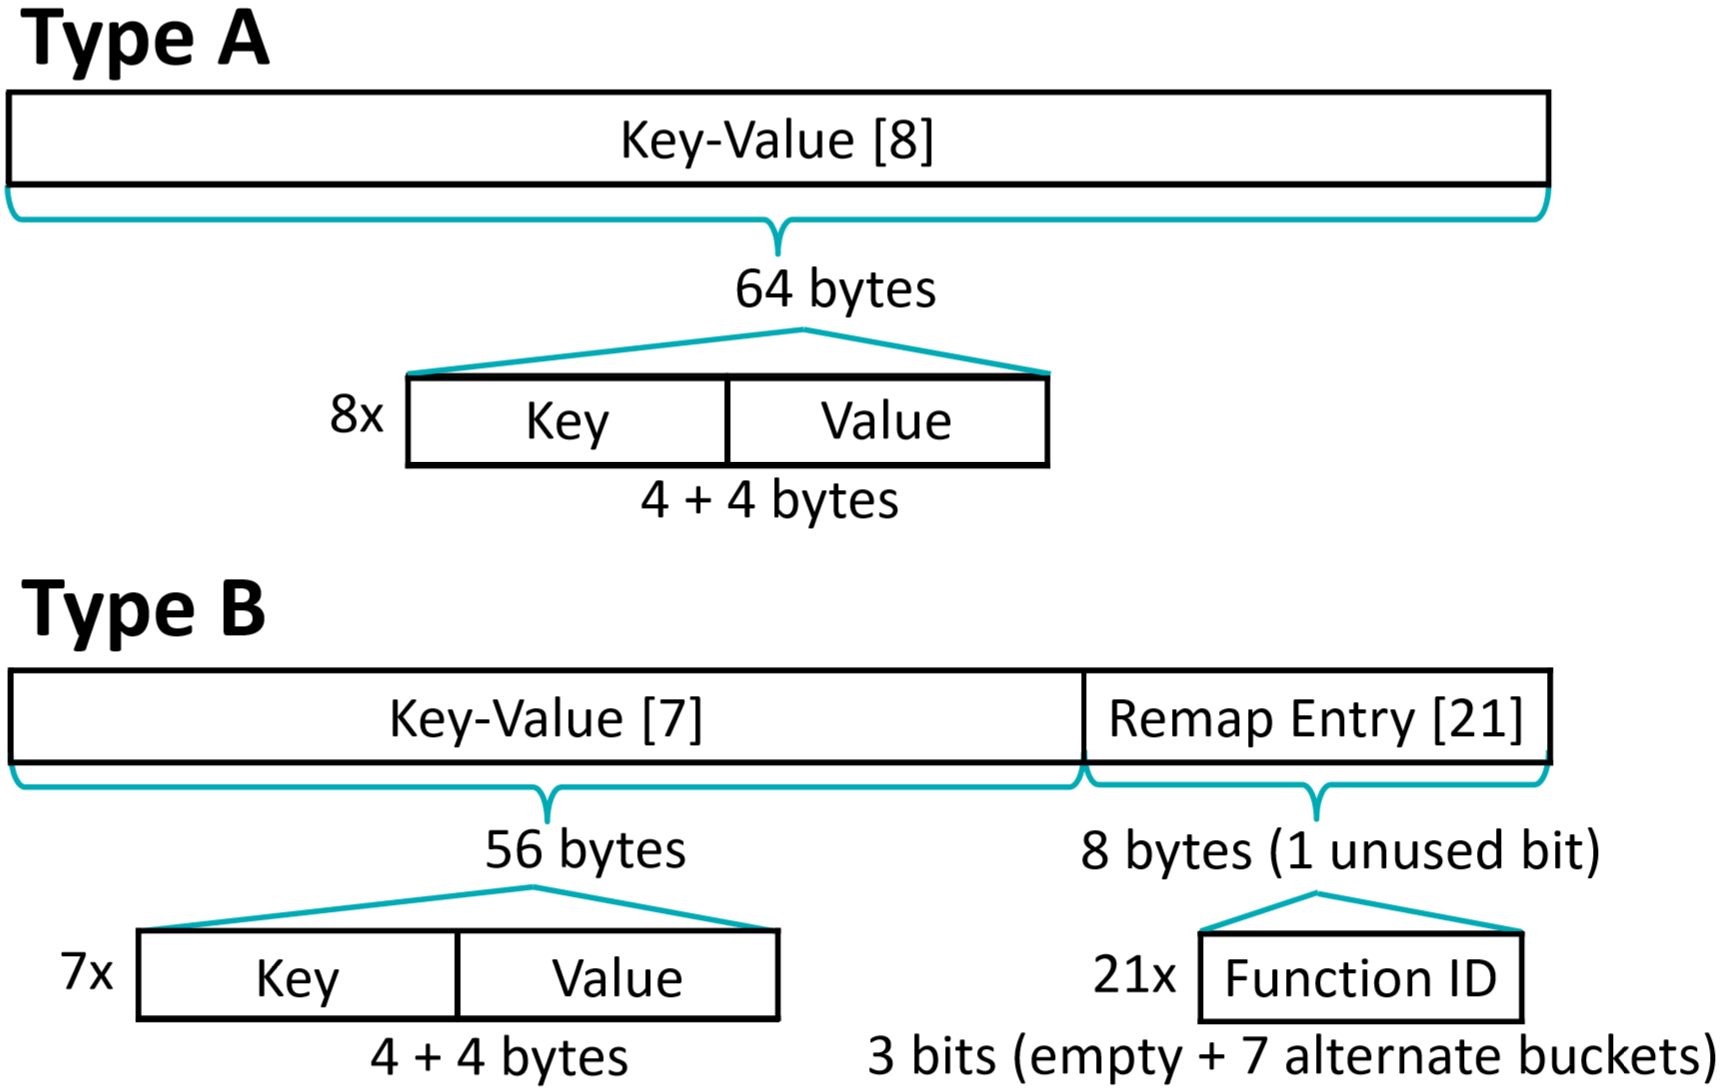
\includegraphics[width=\linewidth]{2-type-buckets.png}
    \caption{Horton tables use 2 bucket variants: Type A (an unmodified BCHT bucket) and Type B (converts final slot into remap entries).} \label{fig:bucket-type}
\end{figure}

In Horton tables, there is a \textbf{primary hash function} $H_{primary}$ which is used to hash the vast majority of items and thus most of the lookups only need to access one bucket. When inserting an item $KV=(K,V)$, Horton tables always hash the item with $H_{primary}$ first, and if the bucket given by $H_{primary}(K)$ can not hold the item directly, then several \textbf{secondary hash functions} are used to remap the item to other bucket. Denote the bucket given by the $H_{primary}(K)$ as $primary bucket$ and the buckets given by secondary hash functions as $secondary buckets$. Also, an item is called $primary items$ if it is stored in its primary buckets, and $secondary item$ if it is remapped to its secondary buckets. Note that there is no correlation between a bucket's type and its primacy. Both type A and type B buckets can simutaneously accommodate both primary and secondary items.

When overflow happens to a type A bucket, it is converted into type B bucket by converting the last slot into a $remap entry array$ which holds $remap entries$. Each remap entry is a vector of $k$-bit vector that encodes the ID of the secondary function used to hash the secondary item that can not be stored in its primary bucket. Each remap entry can take one of $2^k$ different values. 0 is used for encoding an unused remap entry, and 1 to $2^k-1$ are used to encode which of the secondary functions $R_1$ to $R_{2^k-1}$ was used to hash the remapped item. A tag function $H_{tag}$ is also used to determine which remap entry should be used for an remapped entry.

Remap entries track all secondary items so that for each lookup, no matter the the lookup is positive or negative, and no matter how many secondary hash functions are used to rehash secondary items, at most one primary and sometimes a secondary hash function need to be evaluated. At the same time, space for remap entries are only allocated when they are needed after overflow occurs in the bucket.

Figure.~\ref{fig:bucket-type} shows the Type A and Type B bucket design where both key and value are of 4 bytes and each bucket has 8 slots. The bucket type is encoded using one bit of each bucket. So for type A bucket, there is a slot only has 31 bits. And for type B bucket, sicne 21 3-bits remap entries are endcoded into a 64-bit slot, there is an extra bit for bucket type encoding. If there is a value mapped to the 31-bit slot in type A bucket requires all the 32 bits, we can move the item to other slots in the bucket, or remap it to other buckets, making it a secondary item. For convenience, we use the last bit of the last slot in a bucket to encode bucket type, regardless of the bucket type.

\begin{figure}
    \centering
    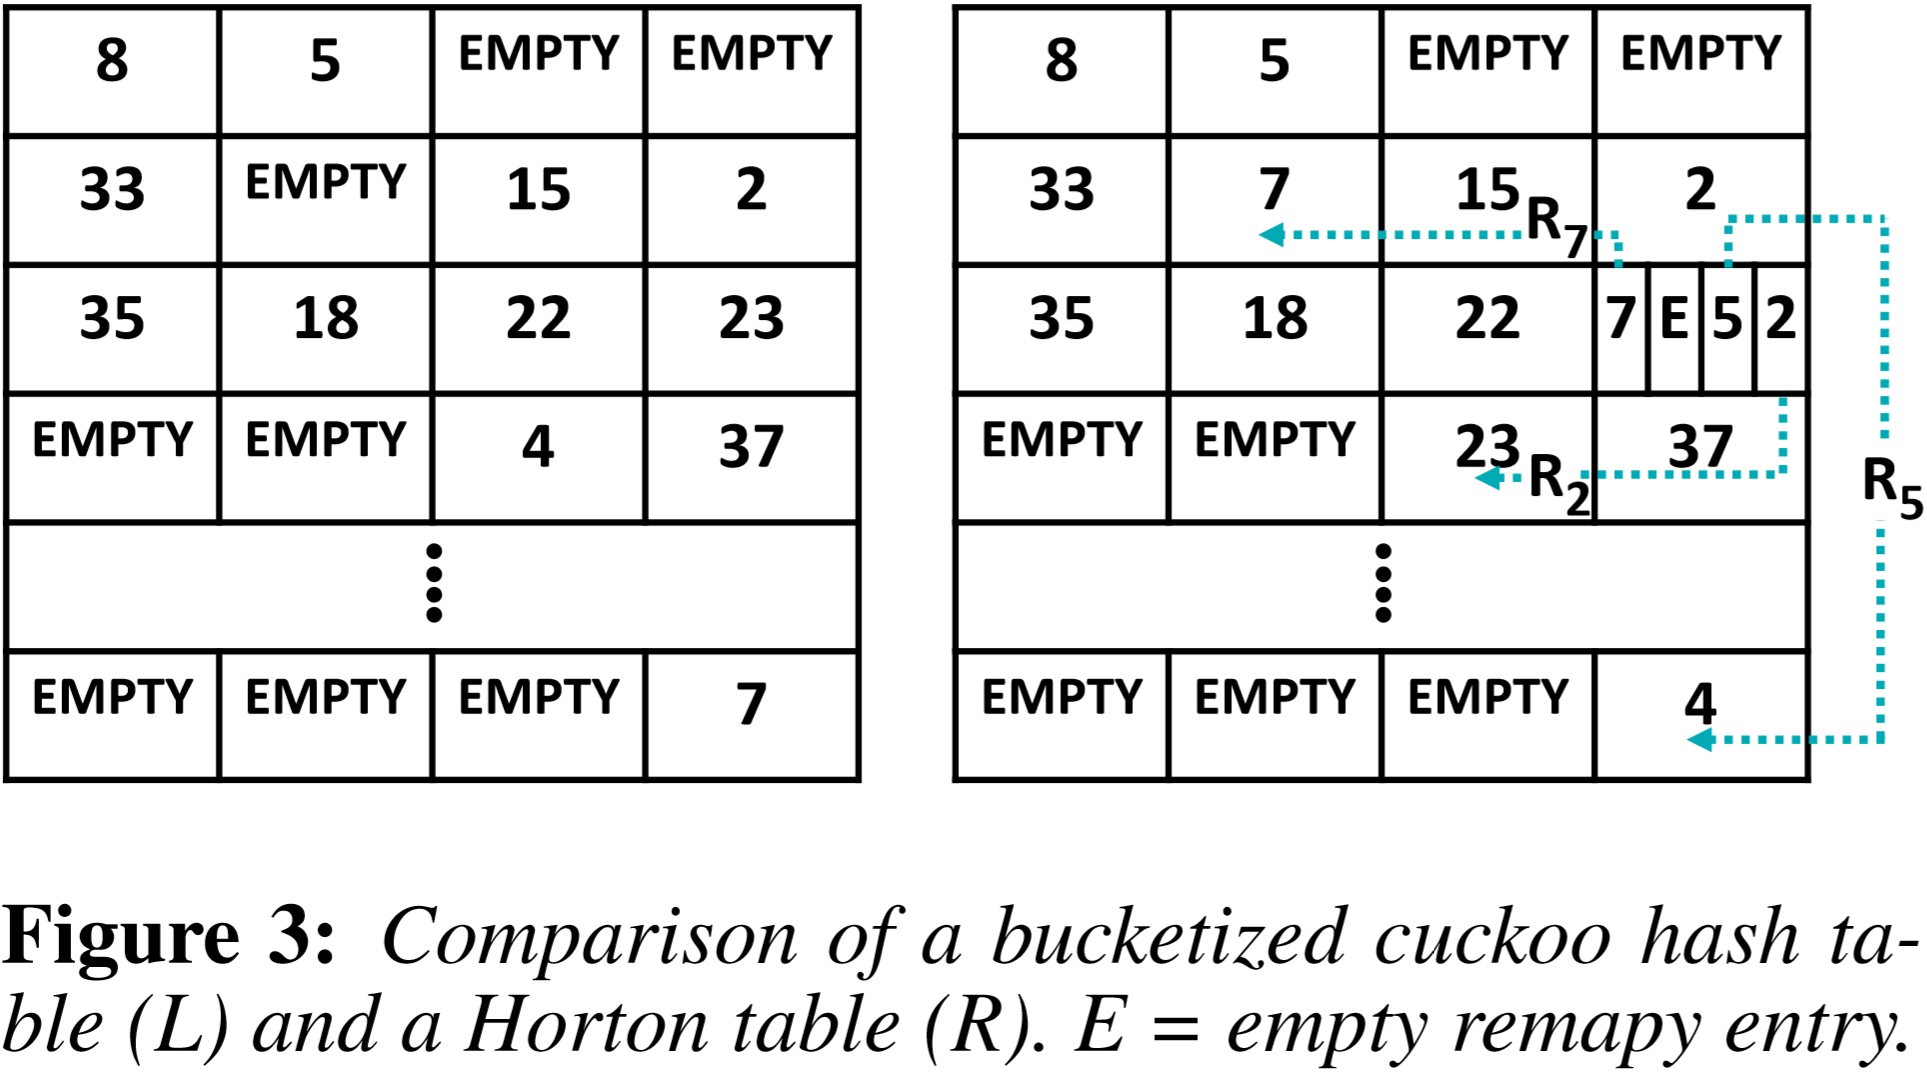
\includegraphics[width=\linewidth]{BCHT-Horton.png}
    \caption{Comparison of a bucketized cuckoo hash ta- ble (L) and a Horton table (R). E = empty remapy entry.} \label{fig:BCHT-Horton}
\end{figure}

Since a type B bucket can hold fewer items than a type A bucket, Horton tables uese as much type A bucket as possible, and a type A bucket is only transformed to type B bucket when there is no sufficient slots to accommodate new comming items, and such process is called $promotion$. And to make sure an item can be found as quick as possible, Horton tables enforce an insertion poliyc that whenever possible, a primary item should not be replaced by a secondary item. With this policy, Horton tables can retain more type A buckets and more primary items. 

Figure~\ref{fig:BCHT-Horton} illustrates the difference between BCHT and Horton tables with $f=2$. Each row corresponds to a bucket and each cell to a slot. In the Horton tables (right one), the third bucket has been promtoed to type B bucket because 4 slots could not hold 6 items (35, 18, 22, 7, 4, 23). Items 35, 18 and 22 are primary items that directly mapped while items 7, 4 and 23 are secondary items and are remapped by hash functions $R_7$, $R_5$ and $R_2$ respectively. If we calculate the lookup costs of two hasing schems, we find that, of the shown buckets, the Horton table has a lookup cost of 1 for elements 8, 5, 33, 15, 2, 35, 18, 22, and 37 and a lookup cost of 2 for 7, 23, and 4, which averages out to 1.25. By contrast the bucketized cuckoo hash table has an expected lookup cost of 1.5 or 2.0, depending on the implementation.

\begin{figure}
    \centering
    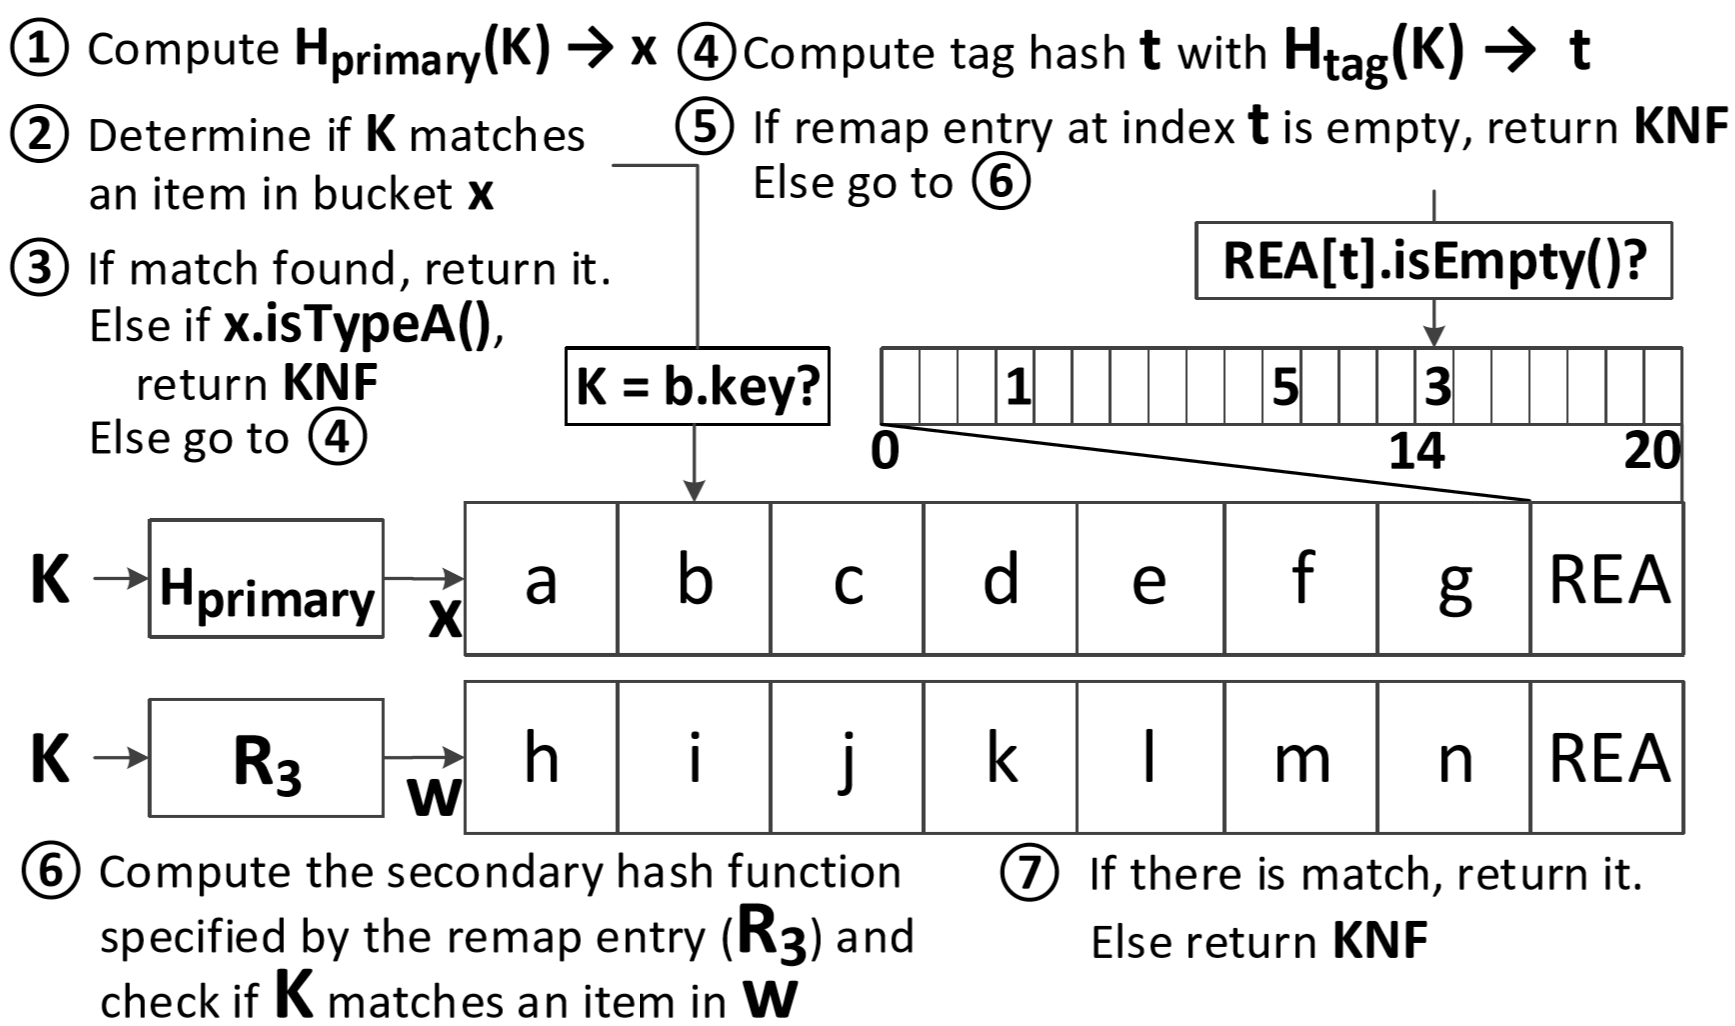
\includegraphics[width=\linewidth]{Horton-lookup.png}
    \caption{Horton table lookups. KNF and REA are ab- breviations for key not found and remap entry array.} \label{fig:Horton-lookup}
\end{figure}

Figure.~\ref{fig:Horton-lookup} shows the lookup algorithm of Horton table. The basic idea is that we first check the first $S$ or $S-1$ slot of the primary bucket of the expected item, depending on whether this bucket is type A or Type B. If we found it, then we are done. In the case that we do not find the item in the primary bucket, if this bucket is type A, then we return the result of negative look up. Othewise, the item may be mapped to othe bucket. We use the $H_{tag}$ function to locate the remap entry of the item, if the entry is empty, then we return the result of negative lookup. Otherwise, we use the hash function wiht the ID given by the remap entry to locate the secondary bucket of the item, and check its existence there.

\begin{figure*}
    \centering
    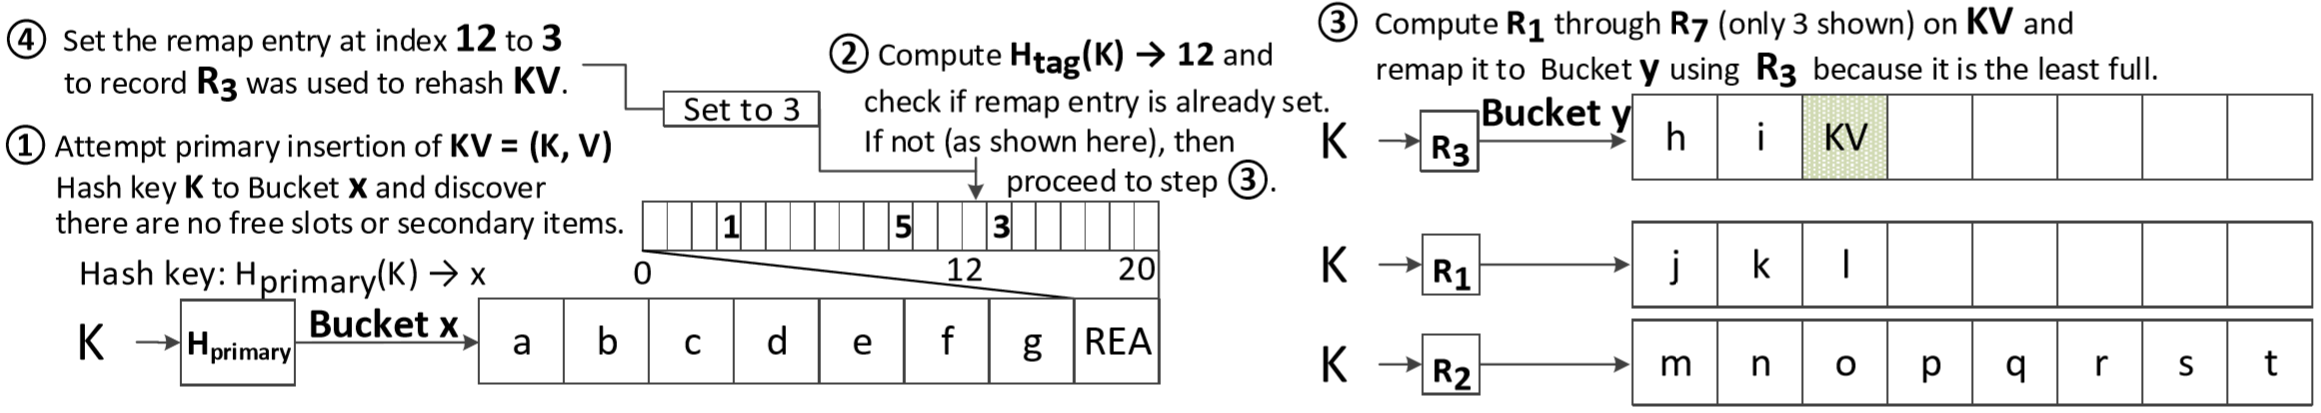
\includegraphics[width=\textwidth]{Horton-insert.png}
    \caption{Common execution path for secondary inserts. REA is an abbreviation of remap entry array.} \label{fig:Horton-insert}
\end{figure*}

The insertion in Horton tables can be classified into two classes: primary insert and secondary insert. The primary insert happens when the primary bucket has an empty slot to hold the item. And if we are not able to place the item into its primary bucket, then a secondary insert is involved. To perform the secondary insert, we first locate the primary bucket using $H_{primary}$. If the primary bucket is not yet a type B bucket, we convert it to a type B bucket. Then we use the $H_{tag}$ to locate the index of remap entry, and then we try out the secondary functions one by one until we find a secondary bucket that can accommodate the item. Finally, we place the item in this secondary bucket and write the ID of the secondary hash function to the remap entry. An table expansion or rehasing is needed if we could not find a slot to accommodate data the item. Fig.~\ref{fig:Horton-insert} shows the algorithm of secondary insert.

\section{Conclusion}
\label{sec:conclude}
Cuckoo hashing introduces a simple hashing scheme that achieves worst-case constant lookup time, which helps storages systems to response to data queries in a real-time manner. However, the kick-out operations of insertion could run into endless loops under unfortunate cases, which makes the insertion performance of cuckoo hashing unpredictable. Many cuckoo hashing variants deal with the endless loops problem by setting an up bound on the number of possible evictions, and perform rehashing if insertion fails. Performing rehashing is expensive, and expected rehashing frequency, although small, may still be unbearable for commercial applications. 

To address the problem, CHS introduces a extra stash to place those problematic items that causing the endless loops, and dramatically reduces the probability that a rehashing is required with the cost of a small memory space for stash. \textit{SmartCuckoo}, on the other hand, points out that the loops of kick-out operations during insertion failures are fruitless efforts and waste substantial resources and time, and it is designed to avoid such useless loops completely. Both CHS and \textit{SmartCuckoo} relies on the properties of cuckoo graph to identify endless loops. While CHS only tracks a small portion of the graph that involved with new item during insertion, \textit{SmartCuckoo} tracks the entire cuckoo graph and present it using a pseudoforest. The insertion throughput performance of \textit{SmartCuckoo} is much better than CHS, however, that performance advantage is traded by a huge memory space cost---extra $O(n)$ memory is required to keep the pseudoforest. And the difference makes CHS and \textit{SmartCuckoo} have different application scenarios: CHS is more suitable for system designs where memory space is valuable such as cache designs, while \textit{SmartCuckoo} is better to be applied in the systems where memory is usually sufficient and the performance is a much important issue.

BCHT is a varinat of cuckoo hahsing that exploids higher load factor at the cost of a small lookup overhead. And to improve the lookup performance of BCHT, Horton tables constructs two type of buckets and leverages on an auxiliary remap entries that remap the items that could not be placed in the primary buckets to secondary buckets. Since the space for the remap entries is allocated only when needed, Horton tables achieve a better lookup performce while keeping the space cost at a low level.

\footnotesize{
\bibliographystyle{acm}
\bibliography{paper}
}
\end{document}


